\documentclass{article}
\usepackage{amsmath}
\usepackage{graphicx}
\usepackage{hyperref}
\hypersetup{
		colorlinks=true,
		linkcolor=blue,
		filecolor=magenta,
		urlcolor=cyan,
		pdftitle={Overleaf Example},
		pdfpagemode=FullScreen,
	}
\usepackage{float}
\floatstyle{boxed} 
\restylefloat{figure}
\title{Verilog notes}
\date{01-29-2023}
\author{Tommy Bui}

\begin{document}
	\maketitle
	\newpage
	\pagenumbering{arabic}

	\tableofcontents
	\newpage

	\section{Verilog Tutorial}

	\href{https://www.chipverify.com/verilog/verilog-tutorial}{Reference to Chipverify} \newline

	\subsection{Lore}
	In the early days of integrated circuits, engineers had to physically draw transistors \& their netlist on paper. As circuits became more complex and larger in scale, this process eventually tedious. Languages such as VHDL \& Verilog were developed to simply the process of describing the functionality of IC and let tools convert the behavior into hardware using combinational \& sequential logic. \newline

	\subsection{How is Verilog useful}
	Verilog creates a level of abstraction that hides the details of its implementation \& technology. \newline

	E.g. the design of a D flip-flop requires the knowledge of the transistor layout in order to achieve an edge-triggered FF, rise/setup time, fall/clk-Q times to latch value onto flop, etc.

	\section{Introduction to Verilog}
	\href{https://www.chipverify.com/verilog/verilog-introduction}{Source}

	A digital element such as a FF can be represented using combinational gates such as NAND or NOR gates. The functionality of a FF is determined based on the layout of such gates. \underline{How the gates have to be connected is usually determined using K-maps} \newline

	Below is an schemetic of a Data flip-flop \& its corresponding truth table. The output, q is asserted only when rstn \& d are both set. \newline

	\begin{figure}[H]
		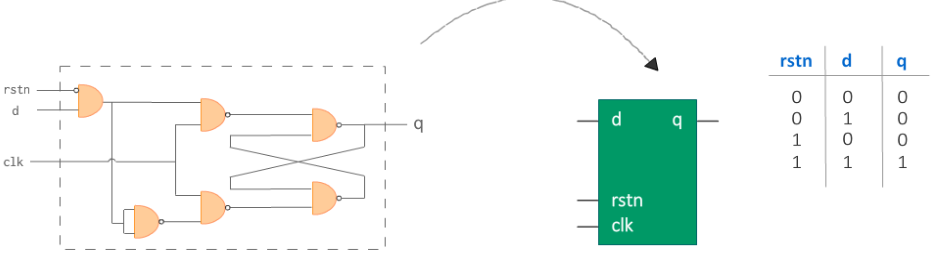
\includegraphics[width=\linewidth]{VerilogPics/figure_1.png}
		\caption{D flip flop}
		\label{D Flip-flop schematic and logic}
	\end{figure}

	\subsection{What is a hardware schematic?}

	A hardware schematic is a daigram that shows how the combinational gates should be connected to implemented a particular behaviour in hardware. From figure 1, a set of NAND gates are connected in order to create a D flip flop. 

	\subsection{What is a Hardware Description Language?}

	It's easier to describe how a block of logic should behave \& let software tools convert that behavior into an actual hardware scchematic. The langugage that describes the hardware functinality is classified as a Hardware Description Language.

	\subsection{Sections of Verilog Code}

	All behavior code should be described within the keywords module \& endmodule. 

	\subsubsection{Verilog section template}
	\begin{itemize}
		\item Module definition \& port list declaration
		\item List of input \& output ports
		\item Declaration of Verilog data types
		\item Module instantiations
		\item Behavioural code
	\end{itemize}

	\begin{figure}[H]
		
\includegraphics[width=\linewidth]{VerilogPics/figure_2.png}
		\caption{Verilog example Template}
		\label{Verilog Template}
	\end{figure}

	\section{Data Types}
	\subsection{Verilog Syntax}

	\href{https://www.chipverify.com/verilog/verilog-syntax}{Source} 
	\href{https://en.wikipedia.org/wiki/Lexical_item}{(Lexical item. In lexicography [citation needed], a lexical item is a single word, a part of a word, or a chain of words ( catena) that forms the basic elements of a language's lexicon (vocabulary)).} \newline \newline

	Lexical conventions in Verilog are similar to C in the sense that it contains a sense of tokens. A lexical token may consist of one or more characters and tokens can be comments, keywords, numbers, strings or white space. However, all lines are terminated by a semi-colon. \newline

	Verilog is case-sensitive, so variables, var\_a \& var\_A differ.


	Two types of comments:
	\begin{itemize}
		\item Single-line comment uses two forward slashes (e.g. //). Single line comments can be nested in a multiple line comment.
		\item Multiple-line comment starts with /* and ends with */ and cannot be nested
	\end{itemize} 
	
	\subsubsection{White space}

	White space refers to spaces, tabs, newlines, \& formfeeds, and is usually ignored by Verilog except when it separates tokens. Be sure to take advantage of this when making readable code. \newline

	\subsubsection{Operators}

	There are three types of operators: unary, binary, \& ternary or conditional. \newline

	\begin{itemize}
		\item Unary operators shall appear to the left of their operand
		\item Binary operators shall appear between their operands
		\item Conditional operators have 2 separate operates that separate 3 operands
	\end{itemize}

	\begin{figure}[H]
		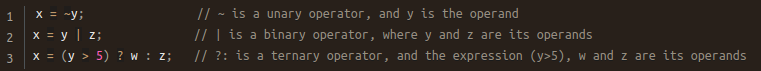
\includegraphics[width=\linewidth]{VerilogPics/figure_3.png}
		\caption{Example of unary, binary, and ternary/conditional operators}
		\label{Example of unary, binary, and ternary/conditional operators}
	\end{figure}

	If the expression (y>5) is true, then variable x will get the value w, else y=z.

	\subsubsection{Number Format}

	\begin{figure}[H]
		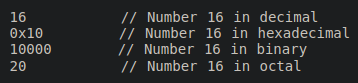
\includegraphics[width=\linewidth]{VerilogPics/figure_4.png}
		\caption{number formats}
		\label{number formats}
	\end{figure}

	By default, Verilog simulators treat numbers as decimals. In order to represent them in different radixes, there are certain rules which must be used. \newline

	\underline{Sized}

	Sized numbers are represented as show below, where size is written only in decimal to specify the number of bits in the number:

	\begin{figure}[H]
		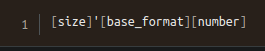
\includegraphics[width=\linewidth]{VerilogPics/figure_5.png}
		\caption{Template for sized numbers}
		\label{Template for sized numbers}
	\end{figure}

	\begin{itemize}
		\item base\_format can be decimal('d or 'D), hex('h or 'H), or octal('o or 'O) \& specifies the base of the number
		\item number can be specified as any valid digit with respect to the specified based format
	\end{itemize}

	\begin{figure}[H]
		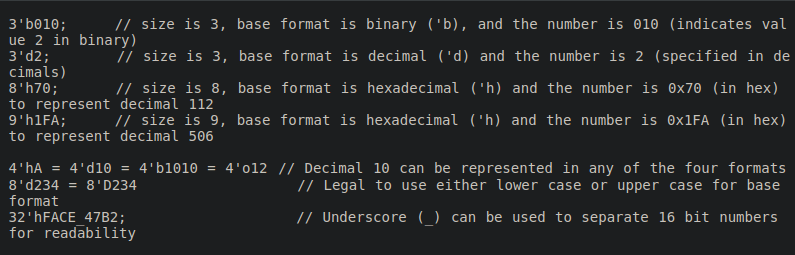
\includegraphics[width=\linewidth]{VerilogPics/figure_6.png}
		\caption{ToDo}
		\label{ToDo}
	\end{figure}

	\subsubsection{Unsized}

	Numbers without a size format specification have a default number of bits depending on the simulator \& machine.

	\subsubsection{Negative} 
	Negative numbers are specified with the - sign before the size of a number; It is illegal to have the - between base format \& number.

	\begin{figure}[H]
		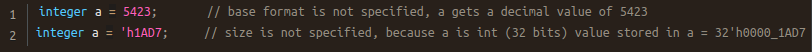
\includegraphics[width=\linewidth]{VerilogPics/figure_7.png}
		\caption{ToDo}
		\label{ToDo}
	\end{figure}
	\subsubsection{Strings} 

	A sequence of characters enclosed in double quotes are strings. It cannot be split into multiple lines \& every chracter in the string takes 1B to be stored:

	\begin{figure}[H]
		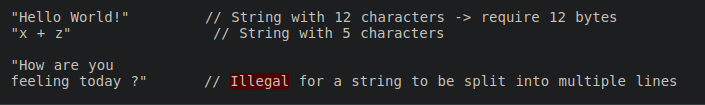
\includegraphics[width=\linewidth]{VerilogPics/figure_8.png}
		\caption{ToDo}
		\label{ToDo}
	\end{figure}
	
	\subsubsection{Identifiers} 

	Identifiers are names of variables; Can be made of alphanumeric characters and symbols. They cannot start with a digit nor a \$:

	\begin{figure}[H]
		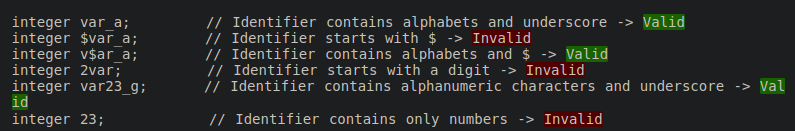
\includegraphics[width=\linewidth]{VerilogPics/figure_9.png}
		\caption{ToDo}
		\label{ToDo}
	\end{figure}

	\subsubsection{Keywords}

	Keywords are special identifiers reserved to be define the language constructs \& are lower case. A list of important keywords is as follows:

	\begin{figure}[H]
		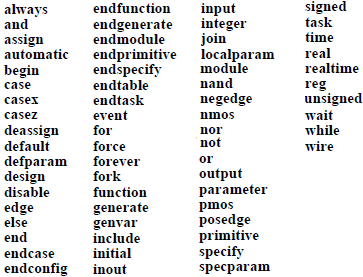
\includegraphics[width=\linewidth]{VerilogPics/figure_10.png}
		\caption{ToDo}
		\label{ToDo}
	\end{figure}

	\subsubsection{Verilog Revisions}
	\begin{figure}[H]
		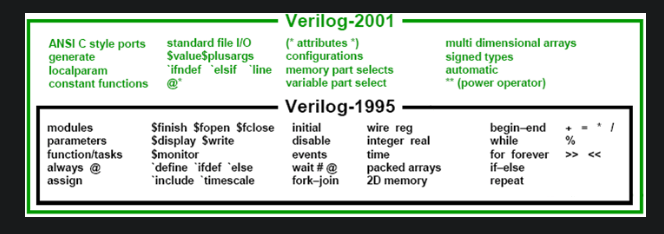
\includegraphics[width=\linewidth]{VerilogPics/figure_11.png}
		\caption{ToDo}
		\label{ToDo}
	\end{figure}




	\subsection{Verilog Data Types}

	\href{https://www.chipverify.com/verilog/verilog-data-types}{Source} \newline \newline

	Data-types in Verilog is meant to represent data storage elements like bits in a flip-flop \& transmission elements like wires that connect between logic gates \& sequential structures. 

	\subsubsection{What values do variables hold?}

	Almost all data-types can have one of the four different values as given below except for \underline{real} \& \underline{event} data types. \newline \newline

	\begin{tabular}{|l|p{6cm}|}
		\hline
		0 & Represents logic zero or false condition \\
		\hline
		1 & Refresents logic one or a true condition \\
		\hline
		x & Represents an unknown logic value (could be 0 or 1, metastability) \\
		\hline
		z & Represents high impedance state \\
		\hline
	\end{tabular}

	The following image shows how these values are represented in timing diagrams \& simulation waveforms. Most simulators use this convention where red stands for X and orange in the middle
	stands for high-impedance or Z. \newline
	:w
	
	\begin{figure}[H]
		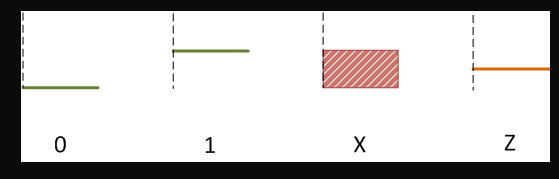
\includegraphics[width=\linewidth]{VerilogPics/figure_12.png}
		\caption{ToDo}
		\label{ToDo}
	\end{figure}

	\subsubsection{What does the verilog value-set imply?}

	Since Verilog is essentially used to describe hardware elements like flip-flops \& combinational logic like NAND \& NOR, it has to model the value system found in hardware. A logic one would
	represent the voltage supply $V_d_d$. \newline \newline

	X or x means that the value is unknown at the time and could either be 1 or 0. This is an issue known as metastability. This differs from the boolean logic X, where it signifies don't care. \newline \newline

	As with any incomplete eletric circuit, the wire that is not connected to anything will have high-impedance at that node which is represented by Z or z. \newline

	\subsubsection{Nets \& Variables}

	Nets \& variables are the two main groups of data types which represent different hardware structures \& differ in the way they are assigned \& retain values. \newline \newline

	\underline{Nets}

	Nets are used to connect between hardware entities like logic gates \& don't store any values on their own. In the follow image, a net\_11 connects between the output of the AND gate and the first
	input of the flip\_floped called data\_0. Similarly, the inputs of the AND gate are connected to nets, net\_45 \& net\_67. \newline

	\begin{figure}[H]
		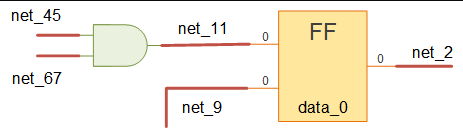
\includegraphics[width=\linewidth]{VerilogPics/figure_13.png}
		\caption{ToDo}
		\label{ToDo}
	\end{figure}

	There are different types of nets with various characterisitcs, the most commonly used net in digital design is of type wire.
Wire is a Verilog data-type used to connect elements \& to connect nets that are driven by a single gate or continuous assignment.

	When there is a requirement for multiple nets, they can be bunched together to form a single wire. In the code below, we can have 
	a 4-bit wire that sends 4 separate values on each one of these wires. A group of such entities is consider a vector. 

	\[ wire [3:0] n0; // 4-bit wire; example of a vector \]

	It is illegal to redeclare a variable name already declared by a net, parameter, or variable. \newline \newline

	\underline{Variables} \newline \newline

	A variable is an abstraction of a data storage element \& can hold values e.g. A flip\-flop. \newline

	Verilog data\-type, reg can be used to model hardware registers since it can hold values between assignments. Note that a reg does not always represent a flip\-flop as it can also represent 
	combinational logic. \newline

	\subsubsection{Other Data\-Types}

	\underline{Integer} \newline \newline 

	\href{https://www.chipverify.com/systemverilog/systemverilog-datatypes}{Properties of data\-types in SV (hopefully same in Verilog)} \newline \newline 

	An integer is a general purpose variable of 32-bits wide which is signed that can be used for other purposes while modeling hardware \& stores integer values.\newline \newline 

	\underline{Time} \newline \newline 

	Time is an unsigned \& 64\-bits wide \& can be used to store simulation time quantities for debugging purposes. A realtime variable simply stores time as a floating point quantity. \newline \newline 

	\underline{Real} \newline \newline

	A real variable can store floating point values \& can be assigned the same way as integer \& reg (See Don Mills' book for properties).

	\subsubsection{Verilog Strings}

	Strings are stored in reg, and the width of the reg variable has to be large enough to hold the string. Each character in a string represents an ASCII value \& requires 1 byte. If the size of the
	variable is smaller than the string, then Verilog truncates teh leftmost bits of the string. If the size of the variable is larger then Verilog appends zeros to the beginning of the string.

	\begin{figure}[H]
		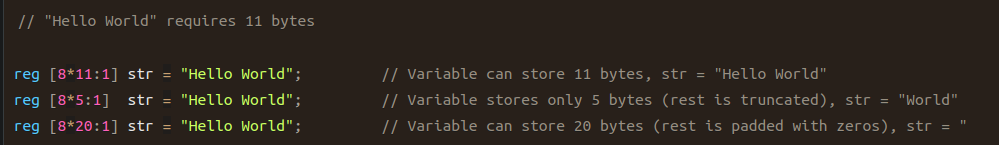
\includegraphics[width=\linewidth]{VerilogPics/figure_14.png}
		\caption{ToDo}
		\label{ToDo}
	\end{figure}

	\subsection{Verilog Scalar \& Vector}

	\href{https://www.chipverify.com/verilog/verilog-scalar-vector}{Reference}
	A single bit can be represented as a flip-flop. However, a 16-bit sequential element is a register that can hold 16 bits, thus Verilog uses scalar \& vector net and variables.

	\subsubsection{Scalar \& Vector}

	A net or reg declaration without a range specification is considered a 1-bit wide scalar. If a range is specified, then the net or reg becomes a multibit entity known as a vector. \newline \newline

	The most significant bit of the vector should be specified as the left hand value in the range while the least significant bit of the vector should be specified on the right.

	\begin{figure}[H]
		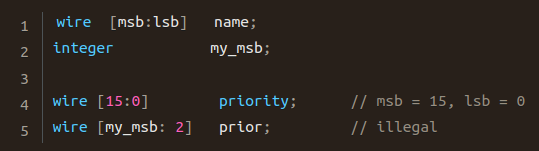
\includegraphics[width=\linewidth]{VerilogPics/figure_15.png}
		\caption{ToDo}
		\label{ToDo}
	\end{figure}

	The msb \& lsb should be a constant expression and cannot be substituted by a variable (if you need to vary the width of vector, consider using parameters). But they can be any integer value -
	positive, negative, or zero; and the lsb value can be greater than, equal to, or less than the MSB.

	\subsubsection{Part-selects}

	A range of contiguous bits can be selected through \underline{part-select}. There are two types of part-selects, one with a constant part-select and another with an indexed part-select. \newlin

	\begin{figure}[H]
		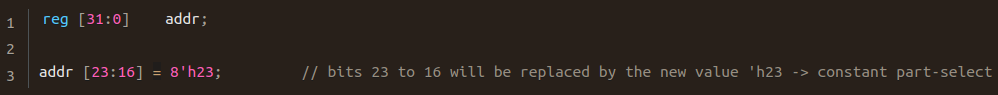
\includegraphics[width=\linewidth]{VerilogPics/figure_16.png}
		\caption{ToDo}
		\label{ToDo}
	\end{figure}

	Using a variable part-select makes it effect to index parts of a vector in loops. Although the starting bit can be varied, the width has to be constant:

	\begin{figure}[H]
		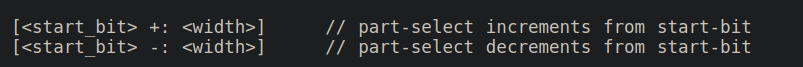
\includegraphics[width=\linewidth]{VerilogPics/figure_17.png}
		\caption{ToDo}
		\label{ToDo}
	\end{figure}

	\begin{figure}[H]
		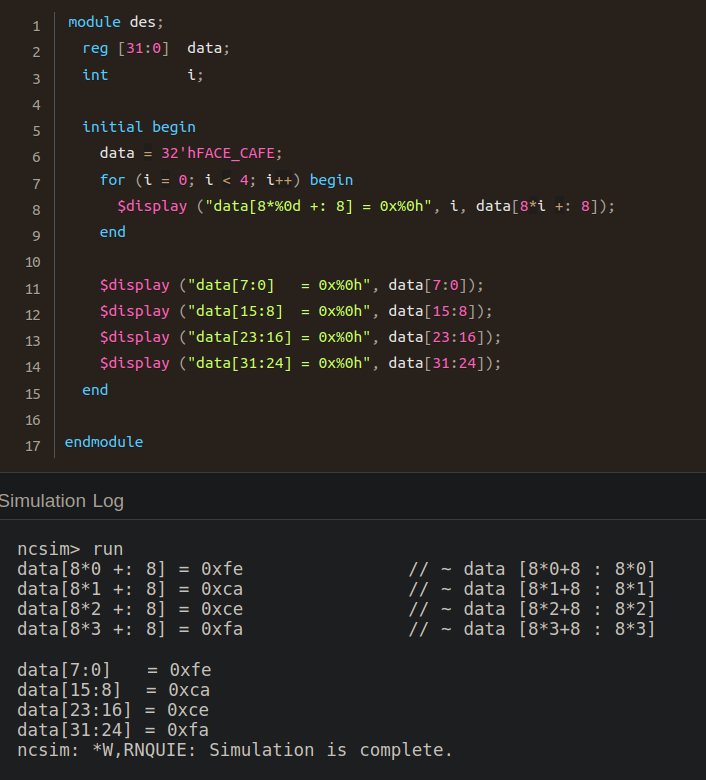
\includegraphics[width=\linewidth]{VerilogPics/figure_18.png}
		\caption{ToDo}
		\label{ToDo}
	\end{figure}

	\subsection{Verilog Arrays \& Memories}

	An array declaration of a net or variable can either be scalar or a vector. Any number of dimensions can be created by specifying an address range after the identifier name. Verilog allows the
	creation of arrays using reg, wire, integer, and real data types.

	\begin{figure}[H]
		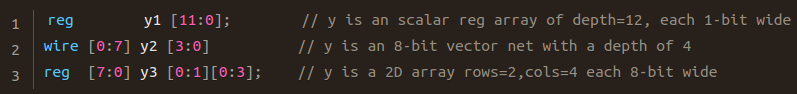
\includegraphics[width=\linewidth]{VerilogPics/figure_19.png}
		\caption{ToDo}
		\label{ToDo}
	\end{figure}

	An index for every dimension has to be specified to access a particular element of an array \& can be an expression of other variables. An array can be formed for any of the different data-types 
	supported in Verilog (note that a memory of N wide 1-bit regs is not the same as an n-bit vector reg). \newline \newline

	\underline{Assignment}

	\begin{figure}[H]
		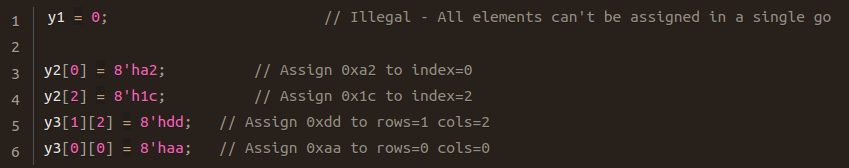
\includegraphics[width=\linewidth]{VerilogPics/figure_20.png}
		\caption{ToDo}
		\label{ToDo}
	\end{figure}

	\subsubsection{Example}

	mem1 is an 8-bit vector, mem2 is an 8-bit array with a depth of 4 (specified by range of [0:3]) \& mem3 is a 16-bit vector 2D array with 4 rows \& 2 columns:

	\begin{figure}[H]
		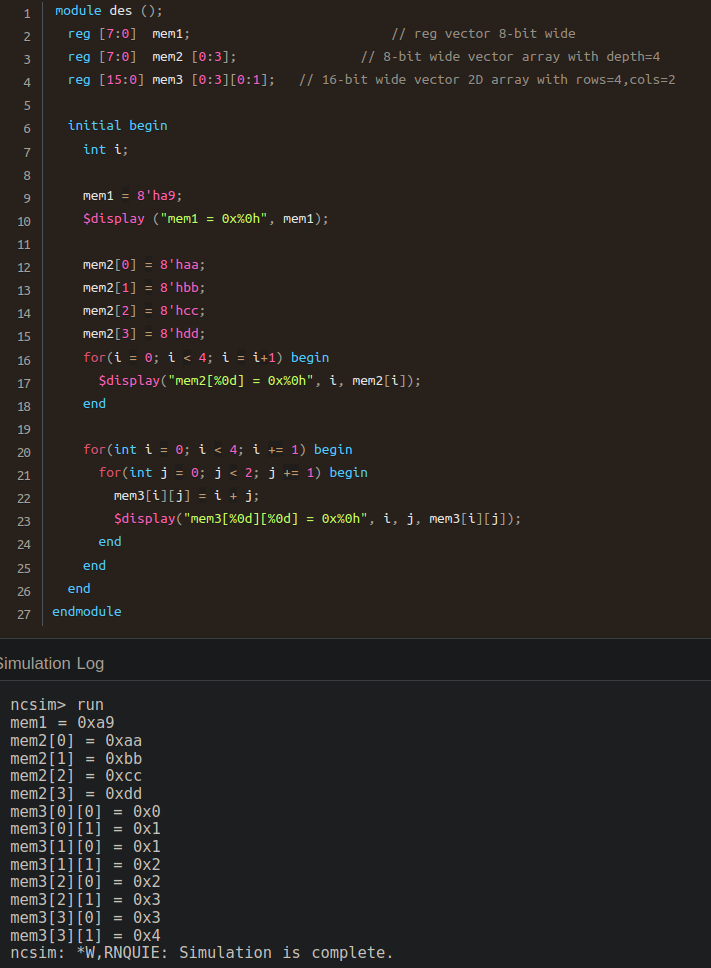
\includegraphics[width=\linewidth]{VerilogPics/figure_21.png}
		\caption{ToDo}
		\label{ToDo}
	\end{figure}

	Notice how the inner loop completes before the outer loop.

	\subsubsection{Memories}

	Memories are digital storage elements that help store data \& information in digital circuits. RAMs \& ROMs are good examples of such memory elements. Storage elements can be modeled using one-dimensional
	arrays of type reg and is called a memory. Each element in the memory may represent a word and is referenced using a single array index.

	\begin{figure}[H]
		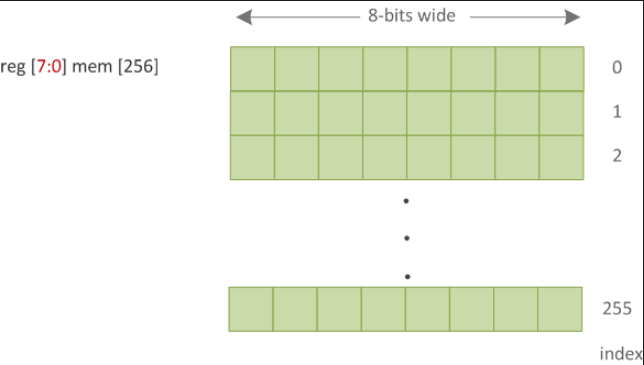
\includegraphics[width=\linewidth]{VerilogPics/figure_22.png}
		\caption{ToDo}
		\label{ToDo}
	\end{figure}

	\subsubsection{Register Vector}
	Verilog vectors are declared using a size range on the left side of the variable name \& these get realized into flops that match the size of the variable. In the code show below, the design 
	module accepts a clock, reset, and some other input signals to RD/WR data into a block. \newline

	It contains a 16-bit storage element called register, which simply gets updated during writes and returns the current value during reads. The register is written when sel \& wr are high on the same
	clock edge. It returns the current data when sel is high \& wr is low:

	\begin{figure}[H]
		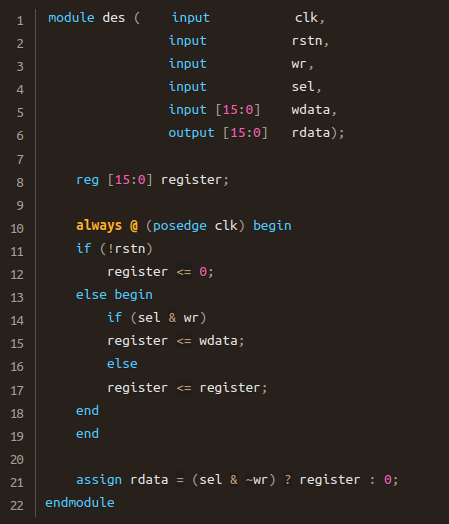
\includegraphics[width=\linewidth]{VerilogPics/figure_23.png}
		\caption{ToDo}
		\label{ToDo}
	\end{figure}
	
	The hardware schematic shows that a 16-bit flop is updated when control logic for writes are active \& the current value is returned when control logic is configured for reads:

	\begin{figure}[H]
		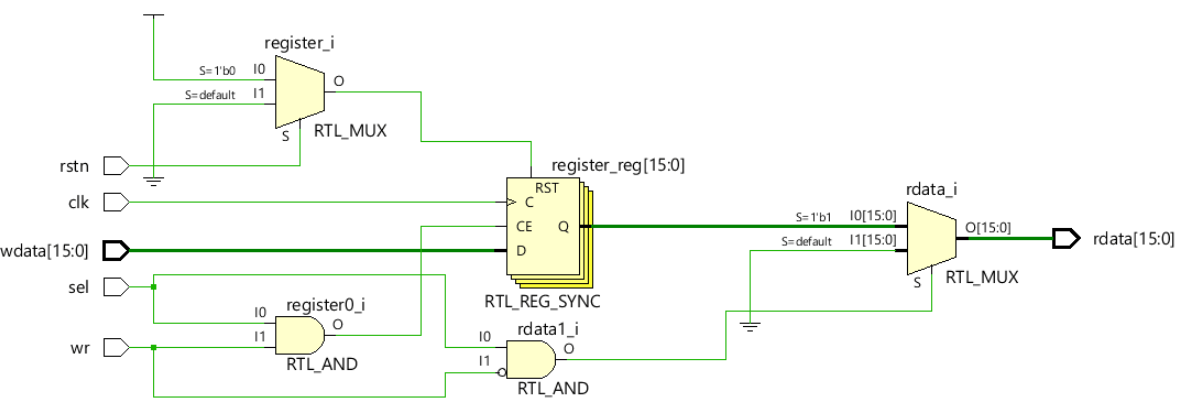
\includegraphics[width=\linewidth]{VerilogPics/figure_24.png}
		\caption{ToDo}
		\label{ToDo}
	\end{figure}

	\subsubsection{Array}

	In this example, register is an array that has four locations with each having a width of 16-bits. The design module accepts an additional input signal which is called addr to access a particular
	index in the array.

	\begin{figure}[H]
		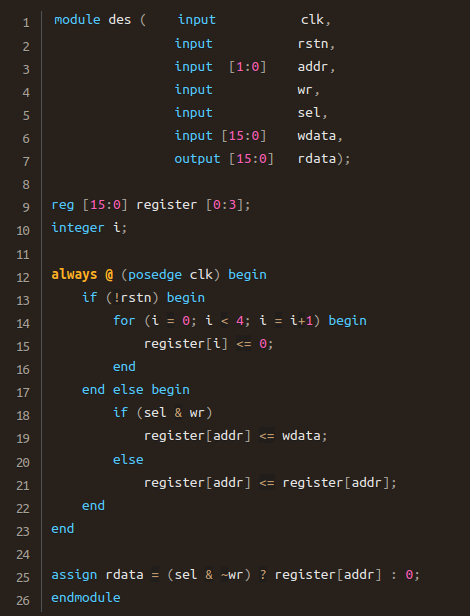
\includegraphics[width=\linewidth]{VerilogPics/figure_25.png}
		\caption{ToDo}
		\label{ToDo}
	\end{figure}

	It can be seen in the hardware schematic that each index of the array is a 16-bit flop and the input address is used to access a particular set of flops.

	\begin{figure}[H]
		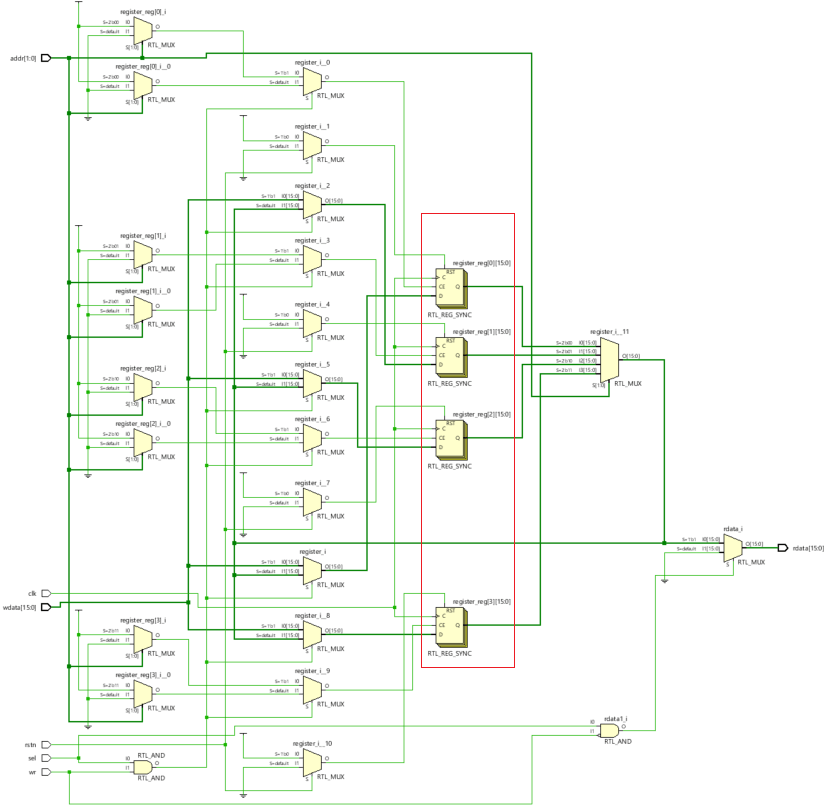
\includegraphics[width=\linewidth]{VerilogPics/figure_26.png}
		\caption{ToDo}
		\label{ToDo}
	\end{figure}

	\section{Building Blocks}	

	\subsection{Verilog Module}

	A module is a block of Verilog code that implements a certain functionality. Modules can be embedded within other modules and a higher level module can communicate with its lower level modules
	using their input \& output ports.

	A module should be enclosed within module \& endmodule keywords. The name of the module should be given after the module keyword as well as a list of optional ports can be declared.

	\subsubsection{Example}

	The module dff represents a D flip-flop which has 3 input ports d, clk, and rstn and one output port, q. The contents within the module block describe how a D flip flop should behave for different
	combinations of inputs. Here, input d is always assigned to output q at posedge of clk if rstn is high.

	\begin{figure}[H]
		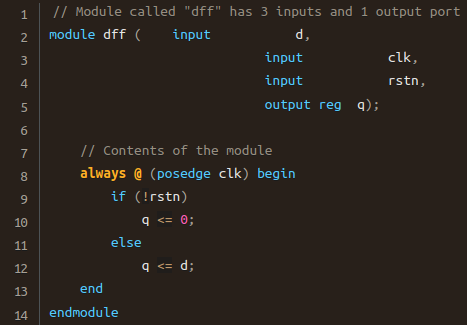
\includegraphics[width=\linewidth]{VerilogPics/figure_27.png}
		\caption{ToDo}
		\label{ToDo}
	\end{figure}

	\begin{figure}[H]
		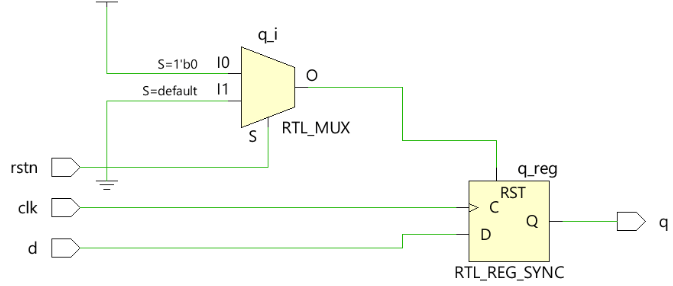
\includegraphics[width=\linewidth]{VerilogPics/figure_28.png}
		\caption{ToDo}
		\label{ToDo}
	\end{figure}

	\subsubsection{What is the purpose of a module?}

	A module represents a design unit that implements certain behavioral characteristics and will get converted into a digital ciruit during synthesis. Any combination of inputs can be given to the
	module and it will providing the corresponding output. This allows such a module to be reused to form bigger modules that implement more complex designs.

	\subsection{Verilog Ports}
	\href{https://www.chipverify.com/verilog/verilog-ports}{Source}

	Ports are a set of signals that define the direction such signals with respect to the module.

	\subsubsection{Types of Ports}

	\begin{tabular}{|l|p{10cm}|}
		\hline
		{\bf Port} & {\bf Description} \\
		\hline
		Input & The design module recieves values using its input port(s) \\
		\hline
		Output & The design module sends values using its output port(s) \\
		\hline
		Inout & The design module can either send or recieve values using its inout port(s) \\
		\hline
	\end{tabular}

	Ports by default are considered as nets of type wire.
	\subsubsection{Signed Ports}
	The signed attribute can be attached to a port declaration or a net/reg declaration or both. Implicit nets are defaulted to unsigned.

	\subsection{Port Variations}

	\underline{Veriog 1995} \newline

	Module declaraions had to frst list the names of its ports withinbrackets and then specify the direction of those ports within the body of the module.

	\begin{figure}[H]
		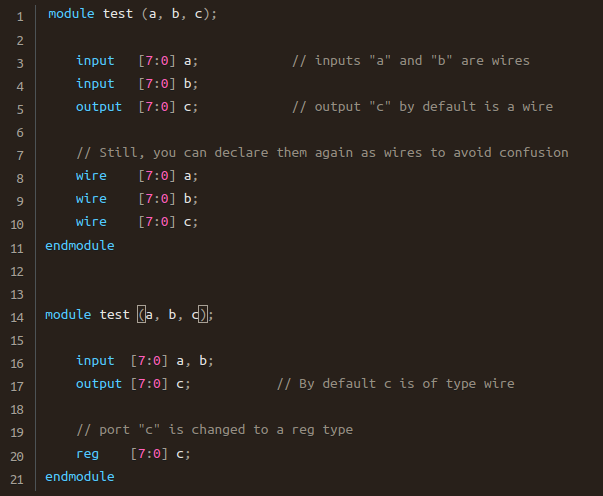
\includegraphics[width=\linewidth]{VerilogPics/figure_29.png}
		\caption{ToDo}
		\label{ToDo}
	\end{figure}

	\underline{Veriog 2001} \newline

	ANSI-C style port naming was introduced in 2001 and allowed the direction to be specified inside the port list.

	If a port declaration is declared as a net or variabled type, then it is illegal to redeclare the same port with another declaration.

	\begin{figure}[H]
		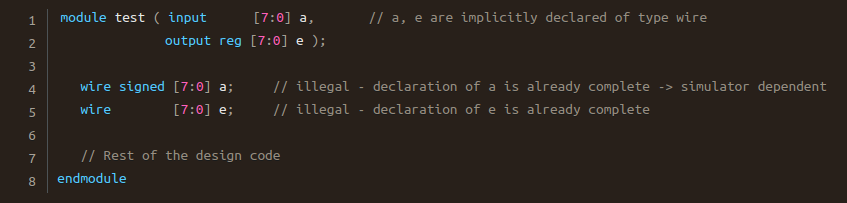
\includegraphics[width=\linewidth]{VerilogPics/figure_30.png}
		\caption{ToDo}
		\label{ToDo}
	\end{figure}

	If the port declaration does not include a net or variable type, then the port can be declared in a net or variable type declaration again.
	\begin{figure}[H]
		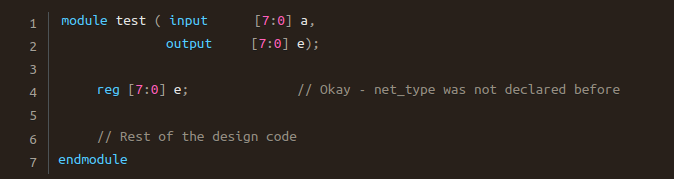
\includegraphics[width=\linewidth]{VerilogPics/figure_31.png}
		\caption{ToDo}
		\label{ToDo}
	\end{figure}

	\subsection{Verilog Module INstnatiations}

	\href{https://www.chipverify.com/verilog/verilog-module-instantiations}{source}

	Bigger and complex designs can be built by integrating multiple modules in a hierarchical manner. Modules can be instantiated within other modules \& ports of these instances can be connected
	with other signals inside the parent module. \newline

	The port connections can be done via an ordered list or by name. \newline

	\subsubsection{Port Connection by Ordered List}

	The connection between the modules can be described by using an ordered list. \newline

	In the following example, mydesign is a module insstantiated with the name d0 in another module called tb_top. Ports are conneted in a certain order which is determined by the position of that port
	in the the port list of the module declaration. For example, b in the testbench is connected to port y of the design simply because both are at the second position in the list of ports in the 
	instantion of d0.

	\begin{figure}[H]
		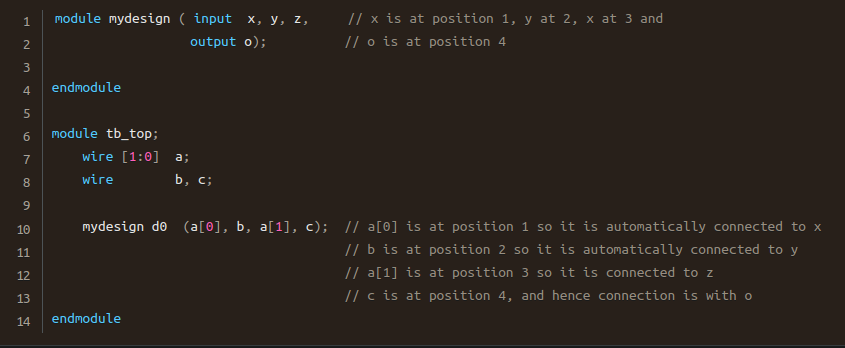
\includegraphics[width=\linewidth]{VerilogPics/figure_32.png}
		\caption{ToDo}
		\label{ToDo}
	\end{figure}

	This method can become inconvenient if the order might change when a new port is added to the list of desired instantiated module or when the number of ports in the design is very large.

	\subsubsection{Port Connection by Name}

	A better way to connect ports is by explicitly linking ports on both sides using their port name.

	The . notation in the port list indicates that the port name following the dot belongs to the design. The signal name to which the design has to be connected is given next within parentheses:

	\[ mydesign d0 ( .x (a[0]), .z(a[1]), .y (a[2]) ); \]

	\subsubsection{Unconected/Floating Ports}

	Ports that are not connected to any wire in the instantiated module will have a state of high-impedance.

	Note that outputs from instantiated modules athat are unconnected are left unconnected in the RTL schematic after sythesis. If the input to such instantiated modules are connected to nets that
	are not being driven than those ports will be grounded in the RTL schematic. \newline

	All port declarations are implicitly declared as wire and hence the port direction is sufficient in that case. However \underline{output ports that need to store values should be declared as reg 
	data type \& can be used in a procedural block like always and initial only}. \newline

	Ports of type input or inout cannot be declared as reg since they're driven from external signals continuously and should not store values. 

	\subsection{Verilog assign statement}

	\href{https://www.chipverify.com/verilog/verilog-assign-statement}{source}

	Signals of type wire or of a similar data type requires a continuous assignment of a value. For example, consider an electrical wire used to connected to different components on a breadboard. As
	long as the power source is connected \& applied to one end of the of the wire, the component connected to the other end of the wire will get voltage. \newline

	In Verilog, this concept is realized by the assign statement where any wire or other similar wire like data-types can be driven continuously with a value. The value may be constant or an expression.

	\subsubsection{Assign Syntax}

	The assignment syntax starts with the keyword assign followed by the signal name which can be a single signal or concatenation of different signal nets. The drive strength \& delay are optional
	\& are mostly used for dataflow modeling than synthesizing into real hardware. The expression or signal on the RHS is evaluated \& assigned to the net or expression of nets on the LHS:

	\[ assign <net\_expression> = [drive\_strength] [delay] <expression or constant value> \] \newline

	Delay values are useful for specifying delays for gates \& are used to model timing behavior in real hardware because the value dictates when the net should be assigned with evaluated value. \newline \newline

	\underline{Rules} \newline \newline

	\begin{itemize}
		\item LHS should always be a scalar or vector net or a concatenation of such nets but never a scalar or vector register
		\item RHS can contain scalar or vector registers \& function calls
		\item Whenever any operand on the RHS changes in value, LHS will be updated instantly with the new value
		\item assign statements are also called continuous assignments \& are always active
	\end{itemize}

	Continuous assignment statements can be used to represent combinational gates in Verilog. \newline

	\underline{Consider the following example}

	\begin{figure}[H]
		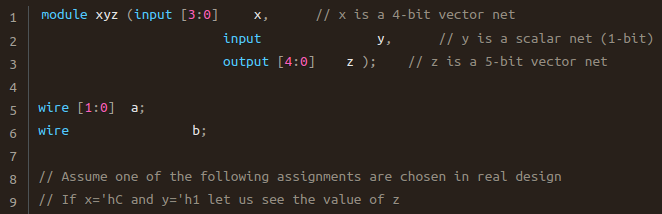
\includegraphics[width=\linewidth]{VerilogPics/figure_33.png}
		\caption{ToDo}
		\label{ToDo}
	\end{figure}

\end{document} 
